
\documentclass[11pt]{article}
\usepackage{acl2014}
\usepackage{times}
\usepackage{url}
\usepackage{amsmath}
\usepackage{latexsym}
\usepackage{graphicx}
\usepackage{algorithm}
\usepackage[noend]{algpseudocode}
\usepackage{appendix}
\usepackage{caption}
\usepackage{framed}
\makeatletter
\def\BState{\State\hskip-\ALG@thistlm}
\makeatother

%\setlength\titlebox{5cm}

% You can expand the titlebox if you need extra space
% to show all the authors. Please do not make the titlebox
% smaller than 5cm (the original size); we will check this
% in the camera-ready version and ask you to change it back.

\title{LING 573 Final Report}
\tiny
\author{Haobo Gu \\
  \small University of Washington \\
  {\tt haobogu@uw.edu} \\\And
 Yuanhe Tian \\
 \small University of Washington \\
  {\tt yhtian@uw.edu}\\\And
 Weifeng Jin \\
 \small University of Washington \\
  {\tt wjin@uw.edu} \\\And
 Haotian Zhu \\
 \small University of Washington \\
  {\tt haz060@uw.edu}\\}

\date{}

\begin{document}
\maketitle
\begin{abstract}

This document discusses the automatic summarization system we built based on various algorithms. Our system takes input as a set of document sets and generates the summarization for each document set. The system has four major parts: data preprocessing, content selection, information ordering and content realization.

\end{abstract}

\section{Introduction}

Automatic summarization is a shared natural language processing task, whose aim is to shorten the input text without losing too much information in the context and create a abbreviated, informative and consistent summary. Generally speaking, there are two approaches for this problem, extraction-based summarization and abstraction-based summarization. The extraction-based method keeps the original sentences while the abstraction-based method generates new sentences for summarization. In this system, we built a system upon the extraction-based method plus compression, which extracts sentences from the input document set and eliminate unnecessary information from these sentences. We used both unsupervised and supervised models for our summarization task and thus prior training on the corpus is required. We used Python3 to implement our system. We evaluated our system using the ROUGE standard and achieved a satisfying performance, with ROUGE-1 F-score as high as 0.30045 and ROUG-4 F-score as high as 0.01679.
\section{System Overview}

We employed the classic system structure for the automatic summarization task, which consists of three major parts: content selection, information ordering and content realization. Since the AQUAINT, AQUAINT-2 and the evaltest corpora have inconsistent data formatting, we add a data preprocessing part to prepare the data. The system flowchart is: \\
\begin{figure}[h]
\begin{center}
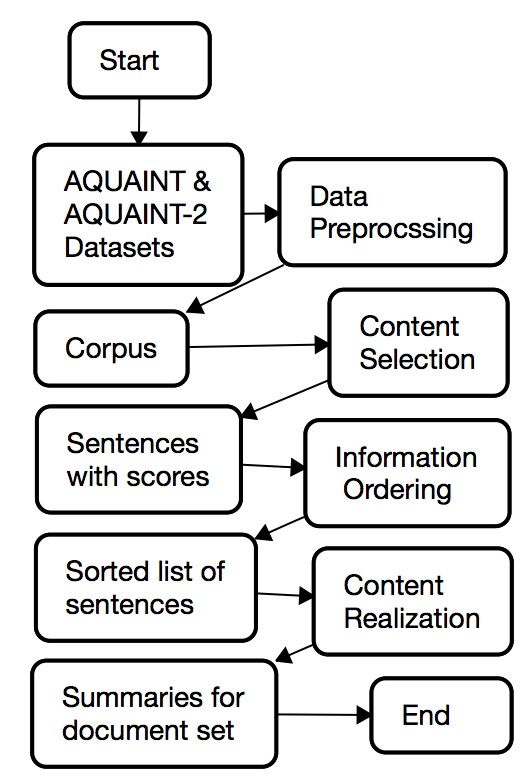
\includegraphics[width=0.37\textwidth]{flowchart.png}
\caption{System Flowchart}
\end{center}
\end{figure}
\indent
The data preprocessing part takes one document specification (one \texttt{.xml} file) and the two corpora as input, and generates a corpus, which includes the list of document sets and a token dictionary to record the frequency of each word occurrence in the input dataset. For each document set in the list, it includes the document set ID, a token dictionary, a topic ID, a collection of summary texts generated by human beings and a list of documents. For each document in the list, it records the document ID, document content, topic ID, a token dictionary, the time of generation and a list of sentences. For each sentence, we record the information of the ID of the document it comes from, the content of the sentence, its position in the document, its score (initialized as 0), sentence length, the time of generation (same as the document) and a token dictionary.\\
\indent
The selection part takes a document set as an input, compresses all the sentences and generates a list of sentences with their scores, computed using a weighted average of several different models. For each document set in the corpus, the part would generate a list of sentences individually.\\
\indent
The information ordering part takes a list of sentences, and returns a sorted list of sentences, using standards of chronology and other measures. \\
\indent
The content realization part takes the sorted list of sentences as input, and removes the unnecessary sentences based on the sentence length and low-rank sentences to generate an output summary for the corresponding document set. The output is a text file and for each document set in the corpus, the system would generate an individual summary text file for it.

\section{Approach}

As mentioned in the Introduction section, our system mainly employs an extraction-based approach. The detailed approach implementation for the three major parts will be discussed below and this approach is targeted to a single document set input.

\subsection{Content Selection}
The content selection part consists a compression part and a scoring part. These two parts rely on two different training sets for model-building and prediction. The system flowchart for content selection is given in Figure 2.
\begin{figure}
\begin{center}
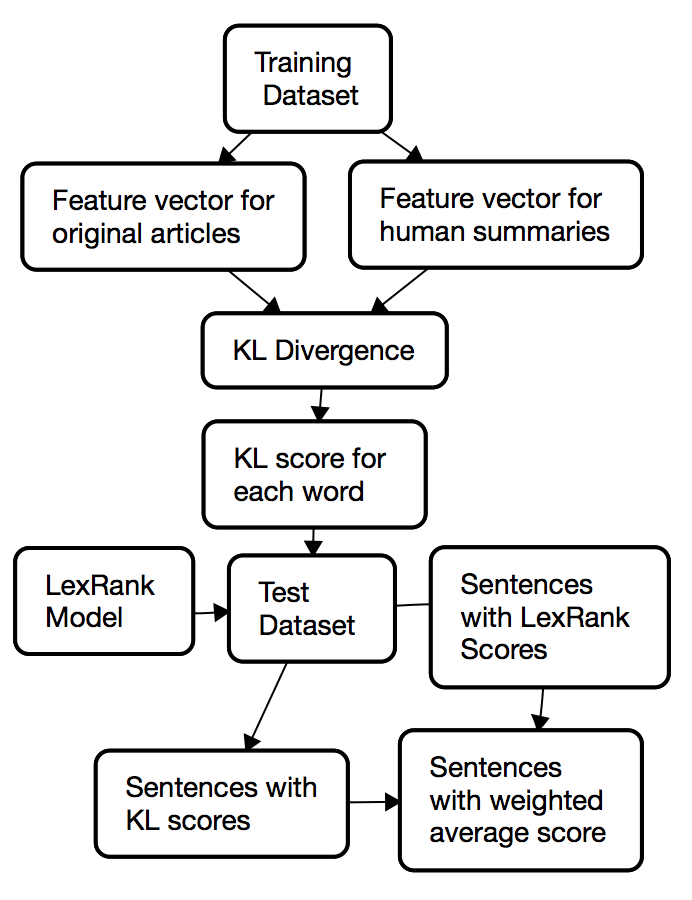
\includegraphics[width=0.4\textwidth]{cs_flow.png}
\caption{Content Selection Flowchart}
\end{center}
\end{figure}

\subsubsection{Compression}
Previously we have tried to use rule-based trimmer compression during the content realization part and the ROUGE-score did not improve significantly. Thus, we decided to apply sequence-labeling models for compression based on Wang's paper (2016) and utilized the compression corpus available on Patas to be our training dataset.\\
\indent
In the feature selection stage, I decided to apply a subset of features used by Wang in his paper, including the word itself, the last 3 letters, the last 2 letters, if it is a stop word, if it is a negative word, its part-of-speech tag and the same information for previous word and next word. I did not use semantic and syntactic features because many of our sentences from the documents are relatively short and some sentences are splitting into two small sentences in some weird ways, which would significantly increase the error rate for parsing and disambiguation.\\
\indent
We want to classify the tokens into 3 labels, O: to be compressed, B: beginning of uncompressed word, I: Inside the uncompressed word. Based on Wang's paper, I used Conditional Random Field algorithm to train my model. I set the L1 penalty coefficient to be 0.1 and L2 penalty coefficient to be 0.01. Also, we set the max iterations to be 500 to avoid over-fitting. The compression results look good as the compression process successfully remove the unnecessary information for summary, including appositives, location information, and time information.  
\subsubsection{Scoring}
Initially, we considered using the method of Log Likelihood Ratio (LLR) and Hidden Markov Model (HMM) to predict if the sentence should be included in the summary based on John Conroy's paper (2004). The paper uses LLR as the HMM feature, and calculates the in-topic frequency and out-topic frequency for each word. In order to make a meaningful training, the training corpus' topics should be at least partially consistent with the test corpus. Unfortunately, the dataset we are using has different distribution of topics in the test and training corpus. \\
\indent
Another difficulty in employing the method is that the HMM requires us to label the sentences in the training dataset as ``in the summary" and ``not in the summary", which requires the training dataset's human summaries to be based on extraction rather than abstraction. Since the summaries we have are all based on abstraction, the approach is very difficult to implement (the only way to achieve that is we label these sentences by hand as the author mentioned in the paper) and thus we abandoned this method. \\
\indent
The first step of our content selection part is to calculate the scores generated by the LexRank model (Erkan and Radev, 2004) and this part can be done without training. Suppose we have $m$ sentences and $n$ tokens in the document set. According to the $tf\times idf$ (Sparck-Jones, 1972) of the token, we can build a feature vector of length $n$ for each sentence and generate a $m\times n$ matrix for the document set, in which each row represents a sentence's feature vector. In addition to that, we compute the cosine distance (based on the LexRank model) for each sentence pair and generate a new $m\times m$ matrix, in which the $ij^{th}$ entry represents the cosine similarity between the $i^{th}$ sentence and the $j^{th}$ sentence. Next, we have to convert the matrix to be a transition probability matrix, in which each row of the matrix would be normalized, and mark this matrix as $M$. \\
\indent
After inspecting our results, the LexRank model turns to assign higher scores on long sentences. Thus, we decided to combined the unsupervised LexRank model and the supervised model based on Kullback-Leibler(KL) divergence (Hong and Nenkova, 2014) to calculate the score for each sentence in the document set, using a weighted average of both models. \\
\indent
The KL model needs a training stage before test. We build two 1-D feature vectors for words in the article and word in summaries. The $i^{th}$ entry in the first vector is $Pr_A(w_i)$, while the $j^{th}$ entry in the second vector is $Pr_S(w_j)$.\emph{w} represents the word to be calculated, \emph{Pr$_S$(w)} represents the probability of \emph{w} appearing in the summaries and \emph{Pr$_A$(w)} represents the probability of \emph{w} appearing in the articles. The probabilities would be logged later to prevent underflow of the system and both vectors would be calculated for the training dataset. \\
\indent
The next step is to calculate the KL score for every word appeared in both articles and summaries in the training data. According to Hong's (2014) research , we calculate both $KL(S||A)$ and$KL(A||S)$ based on the formulas below: 
\begin{equation}
KL(S||A)(w) = Pr_S(w)\ln\frac{Pr_S(w)}{Pr_A(w)}
\end{equation}
\begin{equation}
KL(A||S)(w) = Pr_A(w)\ln\frac{Pr_A(w)}{Pr_S(w)}
\end{equation}
In addition, the value of both $KL(S||A)(w)$ and $KL(A||S)(w)$ will be zero, if either \emph{Pr$_S$(w)} is zero or \emph{Pr$_A$(w)} is zero. \\
\indent
Words with higher $KL(S||A)$ value are more likely to appear in the summary, because Pr$_S$(w) is higher than Pr$_A$(w). And words with higher $KL(A||S)$ value are less likely to appear in the summary, because Pr$_A$(w) is higher than Pr$_S$(w). Therefore, we define the KL score of a word to be the difference between $KL(S||A)$ and $KL(A||S)$, which is shown as following:
\begin{equation}
KL(w) = \frac{(KL(S||A)(w) - KL(A||S)(w))}{2}
\end{equation}
\indent
We store the KL score of every word appearing in the training articles and summaries in a dictionary. Hence, for every word in a given sentence $s$ from test articles, we can get the word's KL score from the dictionary. Then, we will calculate the KL score of that sentence by averaging the KL score of all words. 
\begin{equation}
KL(s) = \frac{\displaystyle\sum_{w_i \in s} KL(w_i)}{length(s)}
\end{equation}
\indent
Now, we find a way to calculate the KL score of a sentence, and the bigger the KL score is, the more likely these words in the sentence will appear in the summary, so that the more important the sentence will be. Therefore, for every sentence in the input document set, we can calculate their KL score and normalize them by the highest KL score of the sentence. The normalized KL score will be the importance score for that sentence.\\ 
\indent
Finally, we generate a 1-D vector $P$,  of length $m$ to record the score of each sentence, in which the $i^{th}$ entry represents the score for the $i^{th}$ sentence. The sentence score is determined by a weighted average of both the LexRank score and KL score. By several trials, we settled down using the weights as 0.25 LexRank Score : 0.75 KL score. In order to avoid short sentences, we remove sentences with length less than 8 words from our output list. \\

\subsection{Information Ordering}

We implement a modified version of the preference learning approach, proposed by Bollegala et al., to provide an ordered list of selected sentences with more readability and meaningfulness. Based on the work by Bollegala et al., we choose the chronological, topic-closeness, precedence and succession experts to compute a quantitative preference of sentence ordering\cite{Bollegala:12}. This sentence ordering procedure proposed in this paper contains five experts in total, but we only adopt four experts since this paper claims that the probabilistic expert hardly contributes to the ordering procedure. 

\indent
Define an expert $e$ by a pairwise preference function as follows:
\begin{equation}
PREF_e(u,v,Q)\in[0,1]
\end{equation}
where $u$ and $v$ are two sentences to order, and $Q$ is the set of sentences that has been ordered so far by some ordering algorithm. Note that the cardinality of $Q$ is 0 when all sentences are unordered. Also, it is worth noting that preference of $u$ to $v$ is not necessarily the same as the preference of $v$ to $u$. 

\indent
Chronological expert orders the sentences in chronological order of publication date, which is defined as follows:
\tiny
\begin{equation}
PREF_{chro}(u,v,Q)=\begin{cases}
				1 & T(u) < T(v)\\
				1 & [D(u)=D(v)]\wedge[N(u)<N(v)]\\
				0.5 & [T(u)=T(v)]\wedge[D(u)\ne D(v)]\\
				0 & otherwise
				\end{cases}
\end{equation}
\normalsize
where $T(u)$ is the publication data of the sentence $u$, $D(u)$ is the unique identification code of the document to which the sentence $u$ belongs and $N(u)$ is the in-text index of the sentence $u$ in its document.

\indent
Topical-closeness expert assumes that in a set of documents pertaining to a broad event, there exists information related to multiple topics. Therefore, to improve readability, sentences of the same or similar topic are to be grouped together. Topical-closeness expert measures the lexical similarity between two sentences by representing each sentence as a vector where if the sentence contains a certain word, then the corresponding value is 1. Topical-closeness expert prefers a sentence which is more similar to the set of sentences that have been already ordered, i.e., sentences in the set $Q$. We define topical-closeness of sentence $l$, $topic(l$) as follows:
\begin{equation}
topic(l)=\underset{q\in Q}{max}\ sim(l,q)
\end{equation}
where we use cosine similarity as the similarity measure between two feature vectors of sentences $l$ and $q$. We also define topical-closeness expert as follows:
\tiny
\begin{equation}
PREF_{topic}(u,v,Q)=\begin{cases}
				0.5 & [Q=\emptyset]\vee[topic(u)=topic(v)]\\
				1 & [Q=\emptyset]\wedge[topic(u)>topic(v)]\\
				0 & otherwise
				\end{cases}
\end{equation}
\normalsize
where $\emptyset$ denotes the empty set, and $u$, $v$ are two sentences to compare preference over.

\indent
In multi-document summarization task with extractive approaches, it is possible that a sentence conveying the main point will be selected in the summary, which however tends to assume information that is not present in selected sentences but in unselected sentences in the original document. Therefore, it is necessary to take information of the unselected sentences in original document to which a selected sentence belongs into consideration. This paper proposes the notion of precedence and succession, which measure preceding or succeeding information of a selected sentence in its original document. We define precedence, $pre(l)$, and succession, $succ(l)$, of a particular sentence $l$ as follows:
\begin{equation}
pre(l)=\frac{1}{|Q|}\sum_{q\in Q}\underset{p\in P_q}{max}\ sim(p,l)
\end{equation}
\begin{equation}
succ(l)=\frac{1}{|Q|}\sum_{q\in Q}\underset{s\in S_q}{max}\ sim(s,l)
\end{equation}
where $q$ is a sentence from the set of sentences that have been already ordered, $P_q$ is the set of sentences that precede sentence $q$ in its original document, and $S_q$ is the set of sentences that succeed sentence $q$ in its original document. We still use cosine similarity for similarity measurement. 

\indent
Finally, with all four experts defined, we define the total preference as follows:
\begin{equation}
PREF_{total}(u,v,Q)=\sum_{e\in E}{w_ePREF_e(u,v,Q)}
\end{equation}
where $e$ is a preference expert from the set of experts $E$, $w_e$ is the learned weight associated with the preference expert $e$, and $u$, $v$, are two sentences to provide preference over.

\indent
By computing total preference of every pair of sentences, we then use the sentence ordering algorithm presented in the same paper to produce the final order of sentences. This ordering algorithm regards the preference function as a directed weighted graph where initially the set of vertices $V$ is equal to the set of sentences $X$, and each edge $u\rightarrow v$ has the weight equal to the preference. Then each vertex $v\in V$ is assigned a potential value $\pi(v)$, which is the sum of outgoing edges minus sum of ingoing edges. This ordering algorithm is a greedy algorithm that orders a certain node $t$ with maximal potential and assigns a rank equal to the cardinality of the set $V$, which then is removed from the graph; also the potential value $\pi$ of the remaining vertices are updated accordingly. This algorithm continues until the graph is empty, i.e., all sentences are ordered. 

\begin{algorithm}
\caption{Sentence Ordering Algorithm.}\label{euclid}
 \hspace*{\algorithmicindent} \textbf{Input:} A set of $X$ of unordered sentences and a preference function $PREF_{total}(u,v,Q)$\\
 \hspace*{\algorithmicindent} \textbf{Output:} Ranking score $\hat{\rho}{(t)}$ of each sentence $t\in X$
\begin{algorithmic}[1]
\Procedure{Ordering}{}
\State $V \gets X$
\State $Q \gets \emptyset$
\For {each $v\in V$}
\State $\pi(v)=\sum_{u\in V}PREF_{total}(v,u,Q)-\sum_{u\in V}PREF_{total}(u,v,Q)$
\EndFor
\While {$V\ne Q$}
\State $t=argmax_{u\in V}\pi(u)$
\State $\hat{\rho}(t)=|V|$
\State $V=V-\{t\}$
\State $Q=Q+\{t\}$
\For {each $v\in V$}
\State {$\pi(v)=\pi(v)+PREF_{total}(t,v,Q)-PREF_{total}(v,t,Q)$}
\EndFor
\EndWhile
\Return $\hat{\rho}$
\EndProcedure
\end{algorithmic}
\end{algorithm}

\indent
This paper also proposed an algorithm for learning weights for each experts. However, training data sets which contain ordered sentences are not available to use. Therefore, we simply used the learned weights in this paper, and we incremented the weight of probabilistic expert to chronological expert since probabilistic expert is not used in our ordering algorithm. Specific weights corresponding to every expert are shown in Figure 3.
\begin{figure}[h]
\begin{center}
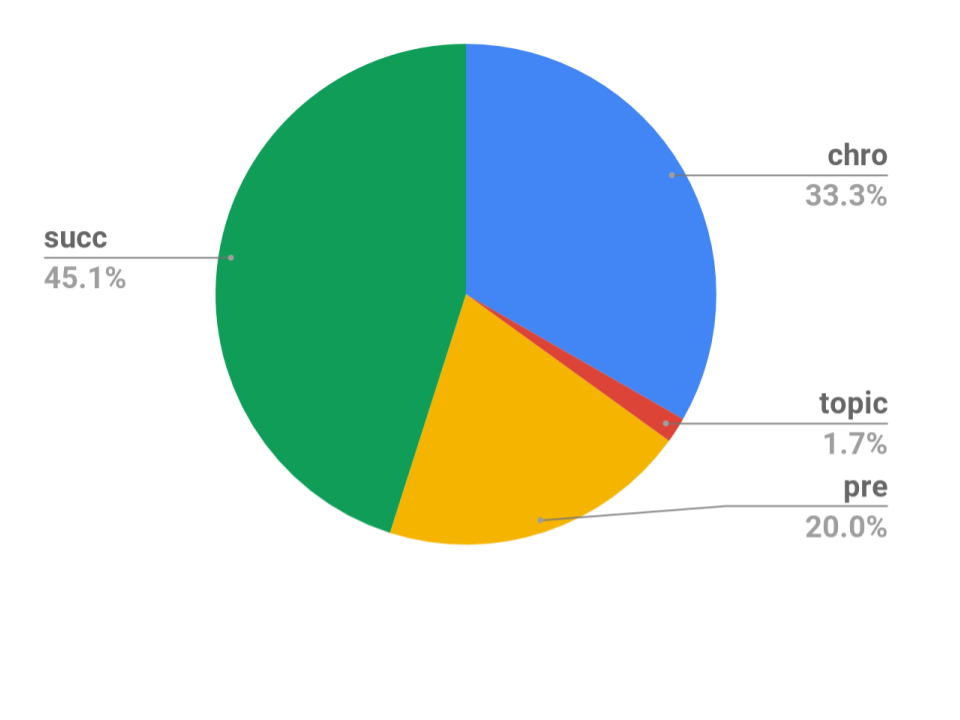
\includegraphics[width=0.45\textwidth]{io_pie.png}
\caption{Weight Percentages of Experts}
\end{center}
\end{figure}


\subsection{Content Realization}

In our content realization module, we implemented an Integer Linear Programming (ILP) method which was proposed by Dan Gillick and Benoit Farve. We use a new objective function which maximizes the weighted summary of all presence bigrams:  
\begin{equation}
	\sum_i{w_ic_i}
\end{equation} 
where binary variable $c_i$ is the presence of bigram $i$ and $w_i$ is the weight. Each bigram has an associated weight, which is the number of document it appears in. Intuitively, the more bigrams appear in the summary, the better the summary is. In our implementation, we modified the target function by removing all bigrams consist of stop-words and punctuations, only meaningful bigrams are considered in the target function. 

Besides presences of bigrams, we also have presences of sentences as variables, which are what we actually want by solving the ILP problem. We have three constraints in our ILP problem. The first constraint is the length constraint:
\begin{equation}
	\sum_j{l_js_j} \leq L 
\end{equation} 
where binary variable $s_j$ is the presence of the sentence $j$, $l_j$ is the length of sentence $j$, and $L$ is the maximum summary length. What's more, we also add a small weight for each sentence variable $s_j$ to reduce the randomness, which is introduced by the ILP algorithm. 

The second and third constraints are about relationships between $s_j$ and $c_i$. Here, we use $Occ_{ij}$ to indicate the occurrence of bigram $i$ in sentence $j$. Obviously, $Occ_{ij}$ is a constant matrix which should be calculated before solving the ILP problem. With $Occ_{ij}$, we can formulate the following constraints:
\begin{equation}
	s_jOcc_{ij} \leq c_i\ \  \forall i,j\label{cons1}
\end{equation}
\begin{equation}
	\sum_j s_jOcc_{ij} \geq c_i\ \  \forall i\label{cons2}
\end{equation}

Constraint (\ref{cons1}) means that if a sentence $j$ is in the summary, then all the bigrams in this sentence would occur in the summary. If sentence $j$ is not in the summary, or bigram $i$ is not in this sentence, this constraint can be always satisfied. Constraint (\ref{cons2}) means that if bigram $i$ is in the summary, then at least one sentence in the summary has bigram $i$. Similarly, if bigram $i$ is not in the summary, constraint (\ref{cons2}) can be always satisfied as well.

Hence, the final ILP problem we established for content realization is:

\begin{equation}
	\begin{aligned}
	\mathrm{Maximize:} & \sum_i{w_ic_i} \\
	\mathrm{Subject\ to:} & \sum_j{l_js_j} \leq L \\
 	& s_jOcc_{ij} \leq c_i\ \ \forall i,j\\
	& \sum_j s_jOcc_{ij} \geq c_i\ \ \forall i \\
	& c_i \in \{0,1\}\ \ \forall i \\
	& s_j \in \{0,1\}\ \ \forall j \\
	\end{aligned}
\end{equation}
\\
\indent
By maximizing the target function, a set of sentences is generated. Finally, those generated sentences are organized to the summary using the order we got from information ordering module.

In our implementation, we also incorporate several sentence compression methods with the ILP content realization approach. All selected sentences are compressed by removing some constituents. We tried three types of removal: clauses starting with an adverb, appositions and contents in parentheses. For each sentence, three compressed sentences are generated. Together with the original sentence, four sentences are added as candidates for summary. We use an extra constraint to ensure that only one sentence in four candidates will be chosen in final summary. 

\section{Results}

We trained our model on the training dataset and test on the devtest dataset and evaltest dataset. After that, we used the ROUGE script to compare the generated summaries and the human summaries (as gold standard). comp is the parameter we are using for content selection part, meaning the ratio of sentences we select for next steps. Due to the randomness of ILP solver, we conducted 5 runs for each dataset. Average ROUGE scores for devtest and evaltest datasets are shown in table \ref{tab:1} and table \ref{tab:2}.\\
\begin{table}[!ht]
\centering
\caption{Average ROUGE Results for devtest (comp=0.1)}\label{tab:1}
\begin{tabular}{|l|l|l|l|}
\hline
ROUGE   & Recall  & Precision & F-score \\ \hline
ROUGE-1 & 0.25908 & 0.28323   & 0.27023 \\ \hline
ROUGE-2 & 0.07042 & 0.07760   & 0.07374 \\ \hline
ROUGE-3 & 0.02342 & 0.02590   & 0.02457 \\ \hline
ROUGE-4 & 0.00851 & 0.00949   & 0.00896 \\ \hline
\end{tabular}

\end{table}
\begin{table}[!ht]
\centering
\caption{Average ROUGE Results for evaltest (comp=0.1)}\label{tab:2}
\begin{tabular}{|l|l|l|l|}
\hline
ROUGE   & Recall  & Precision & F-score \\ \hline
ROUGE-1 & 0.27683 & 0.30468   & 0.28923 \\ \hline
ROUGE-2 & 0.07404 & 0.08163   & 0.07738 \\ \hline
ROUGE-3 & 0.02641 & 0.02897   & 0.02753 \\ \hline
ROUGE-4 & 0.01281 & 0.01390   & 0.01329 \\ \hline
\end{tabular}
\end{table}\\
\indent
Also, we tried to use a high comp rate for test, which means reserving more sentences during the selection part for information ordering and realization. Although the program running time is very long (more than 24 hours), the results show a very strong improvement.\\
\begin{table}[!ht]
\centering
\caption{ROUGE Results for devtest (comp=0.8)}
\begin{tabular}{|l|l|l|l|}
\hline
ROUGE   & Recall  & Precision & F-score \\ \hline
ROUGE-1 & 0.27857 & 0.29007   & 0.28358 \\ \hline
ROUGE-2 & 0.08302 & 0.08615   & 0.08438 \\ \hline
ROUGE-3 & 0.03072 & 0.03163   & 0.03110 \\ \hline
ROUGE-4 & 0.01252 & 0.01267   & 0.01257 \\ \hline
\end{tabular}
\caption{ROUGE Results for evaltest (comp=0.8)}
\begin{tabular}{|l|l|l|l|}
\hline
ROUGE   & Recall  & Precision & F-score \\ \hline
ROUGE-1 & 0.27984 & 0.32699   & 0.30045 \\ \hline
ROUGE-2 & 0.08556 & 0.09919   & 0.09152 \\ \hline
ROUGE-3 & 0.03314 & 0.03792   & 0.03524 \\ \hline
ROUGE-4 & 0.01579 & 0.01808   & 0.01679 \\ \hline
\end{tabular}
\end{table}\\
Our improved system performs far better than our baseline system and previous D3 system, in all ROUGE aspects. The improvement rates are shown below:
\begin{figure}[!ht]
\begin{center}
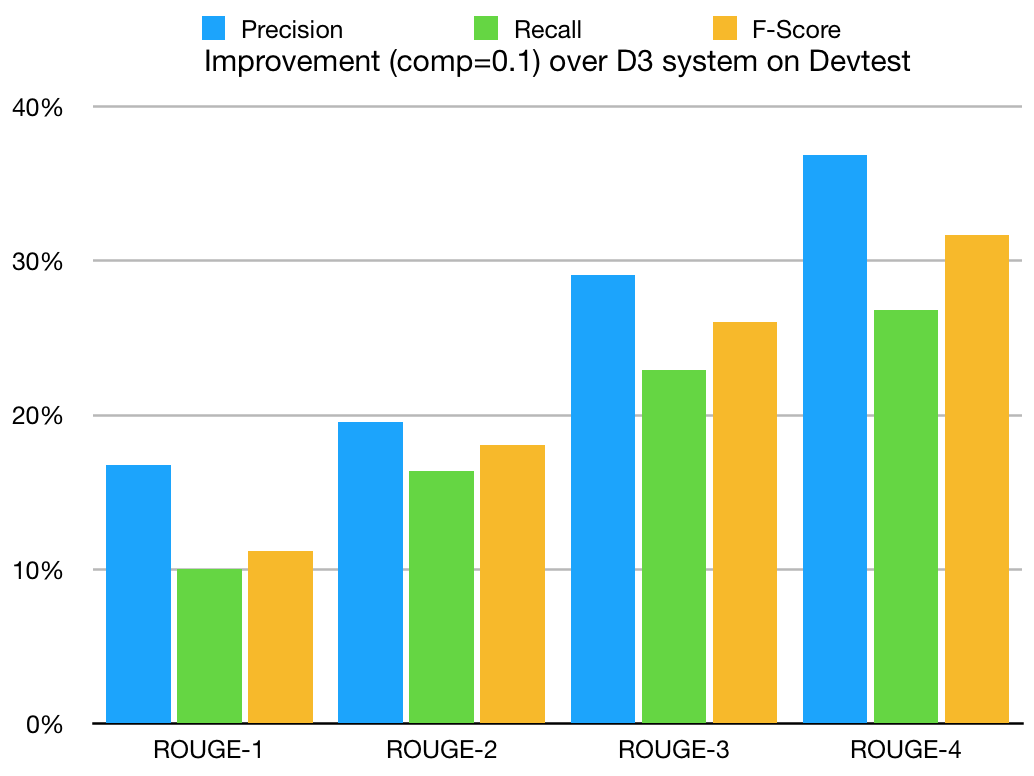
\includegraphics[width=0.33\textwidth]{perc_d4.png}
\caption{Improvement over Deliverable 3}
\end{center}
\end{figure}
\begin{figure}[!ht]
\begin{center}
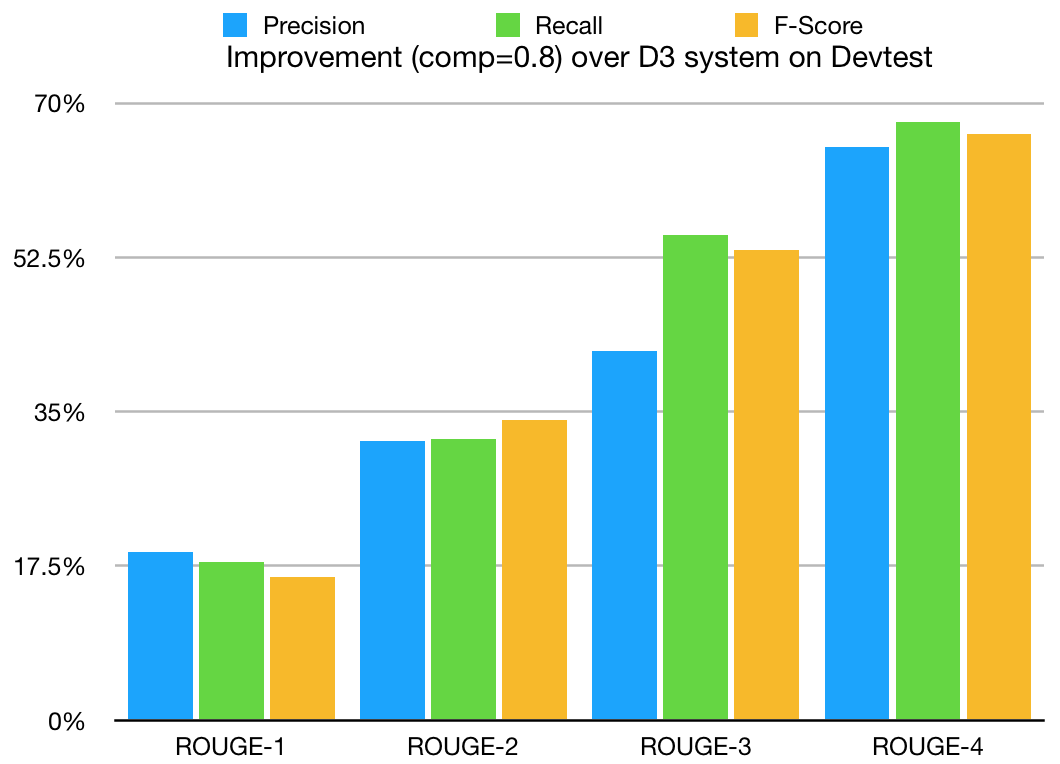
\includegraphics[width=0.33\textwidth]{perc_d4_2.png}
\caption{Improvement over Deliverable 3}
\end{center}
\end{figure}
\section{Discussion}
Based on the improvement chart above, our system improves significantly in all ROUGE standards. 
\subsection{Results Discussion}
Although the improvements of our current system are significant, there are some system flaws that we currently cannot solve. The first problem is that for each time of summarization generation, our system would generate slightly different summaries for a small subset of the test dataset, resulting in a small fluctuation of the ROUGE scores. The problem resulted from the ILP algorithm we used in the Content Realization module. On some occasions, there might be more than 1 solution for the optimization problem and the system would randomly select one optimal sentence for construction. Originally we tried to choose a pseudo-random fixed sentence, but we realize that would not help improve our system performance and decided to keep the small fluctuation in the system.
\indent
Another problem is that this improved system is still primarily extraction-based and does not combine combine different sentences. An abstraction-based system would be more plausible in such task and more similar to the thinking of human beings. We might want to modify our Content Realization part to see if we can build an abstraction-based system in the future.
\subsection{Error Analysis}
Our automatic summarization generates summary for the document set D1003A from the devtest dataset, whose title is Giant Panda:\\
``More than 20 million hectares of forest have been brought under protection and 3.61 million hectares of forest have been planted since 1997 .
The central and provincial governments have invested 160 million yuan 20 million US dollars ) into panda protection programs since .
Nature preserve workers in northwest China 's Gansu Province have formulated a rescue plan pandas from food shortage caused by arrow bamboo flowering .
The nature preserve , occupying about 220,000 hectares has pandas living wild .
In Sichuan and Shaanxi provinces , two other habitats of pandas , arrow bamboo was found blooming ."\\

In general, we think our summary is relatively understandable and reasonably recapitulative. Compared to the human summaries stored in the model directory, we found our summary has the following problems:

\begin{itemize}  
\item The sentences we extracted and compressed from the documents are all topic-related and clustered around select words. However, these sentences do not concur with the human summaries, which means there exists better content selection results for this document set. We may use the topic information to create a better selection.
\item The human summary focused on a more broad topic. For example, it introduces practices and methods offered by the whole Chinese government but our summaries focused on specific local governments' measures.
\item The order of our extracted sentences is not coherent enough for a streamline understanding. The first sentence and the second sentence should be swapped at least.
\item The sentences we extracted and compressed are tokenized, thus the punctuation does not attach to the proceeding word directly, which is no the same as natural human summaries.
\end{itemize}

The following summary is generated by our system based on the document set D1138A from the evaltest dataset. This summary has the lowest ROUGE-1 score in our deliverable:\\

``They to post travel advisories warning China may have been harvested from unwilling donors ; asked states to cease offering follow-up care to patients who had shady organ transplants in China ; and called on foreign doctors to cut ties with their Chinese counterparts suspected of practices .
near death , I 've been forced to face intense , unexpected decisions donations .
At a first-of-its-kind meeting March , UNOS will take a look at hurdles to improving child organ donation , especially for babies and toddlers .
lawmakers want legal advice before acting for inmates who donate ."\\

Admittedly, this summary practice is not successful in providing a shortened understandable texts summarizing the document set. Compared to the human summaries available, we found the following problems:
\begin{itemize}
\item The first sentence contains a pronoun ``they" but it does not have any antecedent so that readers have no idea what/who the pronoun refers to. We might add a coreference resolution part into our system.
\item The second sentence, which has been compressed and extracted from an interview, should not be included in the final summary.
\item The order of sentences does not provide a meaningful reading sequence to the readers and we found this problem prevalent on politics topic.
\end{itemize}


\section{Conclusion}

We employed both unsupervised and supervised models in this improved system. We add the compression part to eliminate unnecessary information from our extracted sentences. The Content Selection part utilizes word count feature vectors and tf-idf, combines LexRank model with KL divergence to calculate the sentence scores. The Information Ordering part uses a modified version of experts method to sort the sentences and the Content Realization part uses ILP to generate the final summary. \\
\indent
Our improved automatic summarization system performs significantly better than our baseline system and D3 system, especially for longer word sequences since the improvements on Rouge-4 and Rouge-3 are more significant. Although we are still having several issues, including the fluctuation in results and extraction without combination problems, we are satisfied with the performance of our new improved system.

\begin{thebibliography}{}
\bibitem[\protect\citename{Bollegala, Okazaki and Ishizuka}2012]{Bollegala:12}
 Danushka~Bollegala, Naoaki~Okazaki and Mitsuru~Ishizuka
\newblock 2012.
\newblock {\em A Preference Learning Approach to Sentence Ordering for Multi-document Summarization.}
\newblock{Information Sciences 2012, 217:78-95.}
 
\bibitem[\protect\citename{Galanis, Lampouras and Androutsopoulos}2012]{Galanis:12}
Dimitrios~Galanis, Gerasimos~Lampouras and Ion~Androutsopoulos.
\newblock 2012.
\newblock {\em Extractive Multi-Document Summarization with Integer Linear Programming and Support Vector Regression.}
\newblock{Proceedings of COLING 2012, 2012: 911-926.}\\

\bibitem[\protect\citename{Gillick and Favre}2009]{Gillick:09}
Dan~Gillick and Benoit~Favre.
\newblock 2009.
\newblock {\em A Scalable Global Model for Summarization.}
\newblock{Proceedings of the NAACL HLT Workshop on Integer Linear Programming for Natural Language Processing, pages 10–18, Boulder, Colorado, June 2009.}

\bibitem[\protect\citename{Georgi}2018]{Georgi:18}
Ryan~A.Georgi
\newblock 2018.
\newblock {\em Lecture of Content Selection and Information Ordering.}
\newblock{in the course LING 573 Spring 2018 in the University of Washington.}

\bibitem[\protect\citename{Conroy, Schlesinger, Goldstein and O'Leary}2004]{Conroy:04}
John~M.Conroy, Judith~D.Schlesinger, Jade~Goldstein and Dianne~P.O'Leary
\newblock 2004.
\newblock {\em Left-Brain/Right-Brain Multi-Document Summarization.}
\newblock{Proceedings of DUC, 2004}

\bibitem[\protect\citename{Hong and Nenkova}2014]{Hong:14}
Kai~Hong and Ani~Nenkova
\newblock 2014.
\newblock {\em Improving the Estimation of Word Importance for News Multi-Document
Summarization.}
\newblock{Proceedings of the 14th Conference of the European Chapter of the Association for Computational Linguistics 2004, 2004:712-721}

\bibitem[\protect\citename{Erkan and Radev}2004]{Erkan:04}
Gunes~Erkan and Dragomir~R.Radev
\newblock 2004.
\newblock {\em LexRank: Graph-based Lexical Centrality as Salience in
Text Summarization.}
\newblock{Journal of Artificial Intelligence Research 22 2004, 2004:457-479}

\bibitem[\protect\citename{Sparck Jones}1972]{Sparck Jones:72}
Sparck Jones, Karen
\newblock 1972.
\newblock {\em A statistical interpretation of term specificity and its application in retrieval}
\newblock{Journal of documentation, 28(1): 11-21}

\bibitem[\protect\citename{Wang, Raghavan, Castelli, Florian and Cardie}2013]{Wang:13}
Lu~Wang, Hema~Raghavan, Vittorio~Castelli, Radu~Florian and Claire~Cardie
\newblock 2013.
\newblock {\em A Sentence Compression Based Framework to Query-Focused Multi-Document Summarization}
\newblock{Proceedings of the 51st Annual Meeting of the Association for Computational Linguistics 2013, 2013:1384-1394}

\end{thebibliography}

\appendix

\section{Experiment Results}

\begin{table}[!ht]
\begin{tabular}{cc}
\begin{minipage}{1.05\linewidth}
\centering
\caption*{ROUGE-1 scores for devtest (comp=0.1)}
\begin{tabular}{|l|l|l|l|}
\hline
Run   & Recall  & Precision & F-score \\ \hline
1 & 0.25985 & 0.28427   & 0.27114 \\ \hline
2 & 0.25729 & 0.27961   & 0.26761 \\ \hline
3 & 0.26038 & 0.28588   & 0.27218 \\ \hline
4 & 0.25712 & 0.28149   & 0.26836 \\ \hline
5 & 0.26075 & 0.28490   & 0.27186 \\ \hline
\end{tabular}
\end{minipage} 

\begin{minipage}{1.05\linewidth}
\centering
\caption*{ROUGE-1 scores for evaltest (comp=0.1)}
\begin{tabular}{|l|l|l|l|}
\hline
Run   & Recall  & Precision & F-score \\ \hline
1 & 0.27646 & 0.30311   & 0.28835 \\ \hline
2 & 0.28090 & 0.30808   & 0.29300 \\ \hline
3 & 0.27827 & 0.30624   & 0.29065 \\ \hline
4 & 0.27324 & 0.30199   & 0.28602 \\ \hline
5 & 0.27530 & 0.30397   & 0.28814 \\ \hline
\end{tabular}
\end{minipage}
\end{tabular}
\end{table}

\begin{table}[!ht]
\begin{tabular}{cc}
\begin{minipage}{1.05\linewidth}
\centering
\caption*{ROUGE-2 scores for devtest (comp=0.1)}
\begin{tabular}{|l|l|l|l|}
\hline
Run   & Recall  & Precision & F-score \\ \hline
1 & 0.07090 & 0.07820   & 0.07428 \\ \hline
2 & 0.06869 & 0.07515   & 0.07169 \\ \hline
3 & 0.07090 & 0.07853   & 0.07443 \\ \hline
4 & 0.06982 & 0.07715   & 0.07319 \\ \hline
5 & 0.07180 & 0.07895   & 0.07509 \\ \hline
\end{tabular}
\end{minipage} 

\begin{minipage}{1.05\linewidth}
\centering
\caption*{ROUGE-2 scores for evaltest (comp=0.1)}
\begin{tabular}{|l|l|l|l|}
\hline
Run   & Recall  & Precision & F-score \\ \hline
1 & 0.07374 & 0.08121   & 0.07702 \\ \hline
2 & 0.07803 & 0.08579   & 0.08144 \\ \hline
3 & 0.07494 & 0.08264   & 0.07831 \\ \hline
4 & 0.07073 & 0.07828   & 0.07404 \\ \hline
5 & 0.07275 & 0.08022   & 0.07607 \\ \hline
\end{tabular}
\end{minipage}
\end{tabular}
\end{table}

\begin{table}[!ht]
\begin{tabular}{cc}
\begin{minipage}{1.05\linewidth}
\centering
\caption*{ROUGE-3 scores for devtest (comp=0.1)}
\begin{tabular}{|l|l|l|l|}
\hline
Run   & Recall  & Precision & F-score \\ \hline
1 & 0.02435 & 0.02695   & 0.02556 \\ \hline
2 & 0.02254 & 0.02475   & 0.02357 \\ \hline
3 & 0.02352 & 0.02612   & 0.02473 \\ \hline
4 & 0.02288 & 0.02548   & 0.02408 \\ \hline
5 & 0.02380 & 0.02618   & 0.02491 \\ \hline
\end{tabular}
\end{minipage} 

\begin{minipage}{1.05\linewidth}
\centering
\caption*{ROUGE-3 scores for evaltest (comp=0.1)}
\begin{tabular}{|l|l|l|l|}
\hline
Run   & Recall  & Precision & F-score \\ \hline
1 & 0.02610 & 0.02865   & 0.02721 \\ \hline
2 & 0.02898 & 0.03175   & 0.03019 \\ \hline
3 & 0.02659 & 0.02917   & 0.02771 \\ \hline
4 & 0.02511 & 0.02763   & 0.02621 \\ \hline
5 & 0.02528 & 0.02766   & 0.02633 \\ \hline
\end{tabular}
\end{minipage}
\end{tabular}
\end{table}

\begin{table}[!ht]
\begin{tabular}{cc}
\begin{minipage}{1.05\linewidth}
\centering
\caption*{ROUGE-4 scores for devtest (comp=0.1)}
\begin{tabular}{|l|l|l|l|}
\hline
Run   & Recall  & Precision & F-score \\ \hline
1 & 0.00946 & 0.01051   & 0.00994 \\ \hline
2 & 0.00783 & 0.00869   & 0.00823 \\ \hline
3 & 0.00841 & 0.00938   & 0.00886 \\ \hline
4 & 0.00830 & 0.00938   & 0.00879 \\ \hline
5 & 0.00856 & 0.00947   & 0.00898 \\ \hline
\end{tabular}
\end{minipage} 

\begin{minipage}{1.05\linewidth}
\centering
\caption*{ROUGE-4 scores for evaltest (comp=0.1)}
\begin{tabular}{|l|l|l|l|}
\hline
Run   & Recall  & Precision & F-score \\ \hline
1 & 0.01249 & 0.01357   & 0.01296 \\ \hline
2 & 0.01467 & 0.01591   & 0.01521 \\ \hline
3 & 0.01282 & 0.01392   & 0.01330 \\ \hline
4 & 0.01210 & 0.01317   & 0.01257 \\ \hline
5 & 0.01196 & 0.01293   & 0.01239 \\ \hline
\end{tabular}
\end{minipage}
\end{tabular}
\end{table}

\end{document}




